\documentclass[a4paper,dutch,11pt]{scrartcl}
\usepackage{mystyle}

\title{Computer Vision}
\subtitle{Head Pose estimation}
\author{Philippe Tanghe \and Li Quan}
%\subject{Verslag}
\date{1 juli 2011}
\bibliographystyle{acm}
\renewcommand{\familydefault}{\sfdefault} 

\begin{document}
\maketitle

%\begin{abstract}

%\end{abstract}
{\small
\tableofcontents}

\clearpage
\section{Inleiding}
Dit verslag bespreekt het project voor het vak Computer Vision. Dit project omvat het ontwerpen van een \emph{head pose estimation} systeem: de pose van een gegeven 2D-afbeelding van een hoofd moet zo nauwkeurig mogelijk geschat worden. Optioneel volgt na het schatten van de pose ook een systeem voor gezichtsherkenning. 

\minisec{Overzicht}
Eerst situeren we het probleem en geven de specificaties waaraan het systeem moet voldoen. 
Vervolgens geven we een korte samenvatting van de verschillende mogelijkheden om dit probleem aan te pakken. 

Hierna bespreken we onze werkwijze, de daarbij gekozen trade-offs en de bijbehorende resultaten. 
Ten slotte geven we mogelijke verbeteringen en uitbreidingen mee.

\section{Specificaties}
De pose van het hoofd bevat heel wat nonverbale informatie~\cite{nonverbal2,nonverbal}. 2D gezichtsherkenningsystemen werken minder goed als geen rekening gehouden wordt met de pose~\cite{overview,facerec}. 

De bedoeling is dus om een systeem te ontwikkelen dat de hoofdpose op een effici\"ente manier kan schatten. We beperken ons echter tot 1 vrijheidsgraad (i.e., ofwel yaw, ofwel pitch, zie figuur~\ref{fig:pitchyawroll}) en beschouwen het probleem als een classificatieprobleem.

\begin{figure}[hbpt] \centering
 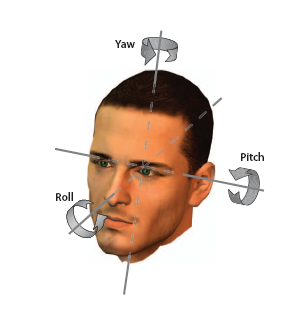
\includegraphics[width=0.25\textwidth]{pitchyawroll}
 \caption{De vrijheidsgraden voor het head pose estimation systeem zijn in dit project beperkt tot ofwel yaw, ofwel pitch. \cite{overview}}
 \label{fig:pitchyawroll}
\end{figure}

De gegeven trainingset bestaat uit gelabelde, hoge-resolutie afbeeldingen (inclusief een aantal landmarks) van de hoofden van een twintigtal personen, elkeen in ieder van volgende poses\footnote{Hierbij komen positieve waarden overeen met een rechtse (yaw) respectievelijk bovenwaartse (pitch) kijkrichting.}:
\begin{itemize}
 \item 0\textdegree{} voor yaw en pitch (neutrale poses).
 \item 10\textdegree{}, 20\textdegree{}, 30\textdegree{}, $\pm$45\textdegree{} en $\pm90$\textdegree{} voor yaw.
 \item $\pm$5\textdegree{} en $\pm10$\textdegree{} voor pitch.
\end{itemize}
(De asymmetrie tussen de linkse en rechtse kijkrichting van de trainingset kan eenvoudig verholpen worden door gebruik te maken van de respectieve gespiegelde versies. In totaal verkrijgen we dus $304$ trainingsafbeeldingen.) 


\section{Overzicht aanpakken}
Eerst geven we een overzicht van de verschillende aanpakken en hun voor- en nadelen, zoals aangegeven in de overview paper \cite{overview}.

\subsection{Appearance template}
Deze methode vergelijkt een nieuwe afbeelding van een hoofd met een verzameling van gelabelde afbeeldingen en zoekt de meest gelijkaardige pose. Dit is een zeer eenvoudig concept en is te gebruiken voor zowel hoge en lage resoluties. 

Het grote nadeel van deze aanpak is dat ze allicht te na\"{\i}ef is. Ze is namelijk gebaseerd op de foutieve veronderstelling dat gelijkaardigheid van afbeeldingen gelijkaardigheid van poses impliceert. Een ander nadeel is dat wanneer de trainingset uitgebreid wordt dat er in principe met steeds meer afbeeldingen moet worden vergeleken, waardoor het systeem steeds rekenintensiever wordt.
% Wanneer er 3 afbeeldingen zijn waarbij 2 van dezelfde persoon zijn met dezelfde belichting maar met een verschil in pose van 5 \textdegree.

\subsection{Detector array} 
Een detector array traint een reeks head detectors die elk afgesteld zijn op een bepaalde pose.
De nieuwe afbeelding krijgt dan als schatting de pose die overeenstemt met de detector(s) die de beste support heeft (hebben). Deze aanpak werkt voor hoge en lage resoluties en kan de uitzicht-eigenschappen (niet pose gerelateerd) van het hoofd leren negeren.

Deze aanpak is discreet van aard en is dus enkel aangewezen voor een beperkt aantal mogelijkheden. (De rekencomplexiteit stijgt lineair met het aantal detectors). Het trainen van de verschillende detectors is vrij moeizaam. Als twee detectors ingesteld zijn voor twee heel gelijkaardige poses, moeten de positieve trainingsvoorbeelden voor de ene negatieve zijn voor de andere (en vice versa). Verder moet er voor elke detector een trainingset zijn die voldoende groot is. %Het gegeven aantal voorbeelden is echter beperkt in aantal per pose.
% Elke detector kan ook het onderscheid maken tussen hoofd en niet-hoofd, waardoor een aparte hoofd-detectie en -lokalisatiestap niet nodig is.

\subsection{Nonlinear regression} 
Deze methode gebruikt niet-lineaire regressietools om een mapping te zoeken van de afbeelding (of de daaruit afgeleide feature data) tot een pose. De meest gebruikte zijn neurale netwerken en recentelijk ook support vector machines \cite{blockeel}. 

Het is niet altijd duidelijk of een goede mapping kan geleerd worden, maar uit de literatuur blijkt dat deze regressietools zeer goed presteren, zowel qua performantie en nauwkeurigheid. Deze systemen zijn wel vrij gevoelig aan de positie van het hoofd in de afbeelding. 

\subsection{Manifold embedding}
Bij manifold embedding zoekt men laagdimensionale manifolds die de variatie in pose modelleren. Het is dus --- meer dan in de vorige methode --- belangrijk een goede dimensionaliteitsreductie te vinden die zoveel mogelijk eigenschappen van de pose behoudt en zo weinig mogelijk karakterspecifieke eigenschappen. Dit is echter niet vanzelfsprekend: methodes hiervoor zijn bijvoorbeeld PCA, KPCA, LDA en KLDA.

Nieuwe afbeeldingen worden dan geprojecteerd in deze laagdimensionale manifolds waarop vervolgens gelijkaardige technieken als voorgaand worden gebruikt.
% Een nadeel is dat deze aanpak enkel aangewezen is voor een beperkt aantal poses.

\subsection{Flexible model}
Deze methode maakt gebruik van landmarks: dit zijn aanduidingen op de afbeelding die overeenstemmen met gezichtspecifieke posities, zoals de ooghoeken. Deze set landmarks vormen een niet-rigide model van het hoofd, dat een bepaalde graad van variatie toelaat.

De pose van een nieuwe afbeelding kan dan geschat worden door de verschillende modellen te vergelijken aan de hand van bijvoorbeeld hun parameterinstantiatie. Een bijkomend voordeel van deze methode is dat ze ook toelaat om virtuele gezichten te genereren (bijvoorbeeld een frontaal gezicht cre\"eren aan de hand van een profielfoto).

\subsection{Geometric model}
Geometrische modellen gebruiken de locatie van een beperkt aantal gezichtskenmerken (bijvoorbeeld ogen en neus). Uit hun relatieve positie kan dan vrij eenvoudig de pose geschat worden. Hierbij kan dus rechtstreeks gebruik gemaakt worden van bepaalde gekende eigenschappen van verschillende hoofdposes.

Voor deze methode moeten de gezichtskenmerken aangeduid zijn of kunnen gedetecteerd worden. Deze methode is dus problematisch wanneer bepaalde gezichtskenmerken moeilijk zichtbaar zijn.

\subsection{Tracking}
Tracking gebruikt videoframes om de verandering in pose te schatten. Deze techniek is dus niet relevant voor dit project waarbij de pose van statische afbeeldingen moeten geschat worden. %De afbeeldingen zijn ook niet te ordenen in een volgorde zodat deze als frames kunnnen worden ge\"{\i}nterpreteerd van een opname van een vloeiende beweging.

\subsection{Hybride}
Hybride methodes combineren meerdere van bovenstaande technieken om zoveel mogelijk de voordelen van verschillende systemen te bundelen en/of nadelen van \'e\'en bepaald systeem te beperken. Het nadeel van deze methode is dat ze meer rekenkracht vergt en dat bij tegensprekende resultaten van verschillende systemen er een keuze gemaakt moet worden.

\section{Hoofdpose schatting}
Voor het maken van de head pose estimator hebben we uiteindelijk gekozen voor het niet-lineaire regressiemodel.
\subsection{Keuze aanpak}
De belangrijkste motivatie voor onze keuze is dat de studies erop wezen dat neurale netwerken (NN) en support vector machines (SVM) heel goede resultaten behalen, zowel op vlak van performantie als nauwkeurigheid. 

NNs worden reeds lang succesvol gebruikt in diverse pattern recognition taken. SVMs zijn recentelijk aan een grote opmars bezig --- niet alleen in de Computer Vision wereld. Bijgevolg hebben deze tools een goede ondersteuning. De nadelen die opgesomd werden, zijn weinig relevant voor dit project (zo zijn de locaties van de hoofden in de afbeeldingen consistent).

In tegenstelling tot neurale netwerken hebben SVMs een betere theoretische basis \cite{theoretical} en is het basisconcept heel elegant, zoals figuur~\ref{fig:svm} illustreert.

\begin{figure}[hbpt]\centering
 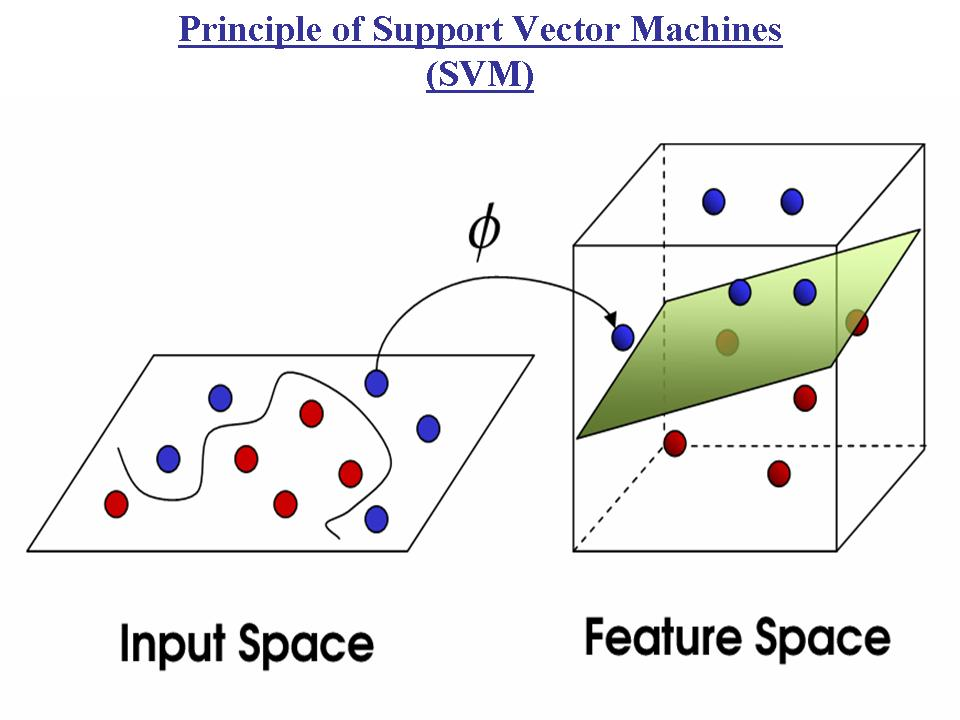
\includegraphics[width=0.65\textwidth]{svm}
\caption{Het principe van een Support Vector Machine. De transformatie naar de hoogdimensionale ruimte (via de kernel trick) laat toe om eenvoudig een hypervlak te zoeken dat de twee klassen lineair scheidt. \cite{svmwikipedia}}
\label{fig:svm}
\end{figure}

\subsection{Overzicht}
We hebben zowel een systeem gebaseerd op neurale netwerken als een op SVMs ontwikkeld. De implementatie is gebaseerd op volgende papers: \cite{neural} en \cite{svmli}.
Voor elk van deze methodes zijn 3 belangrijke onderdelen te onderscheiden: 
\begin{itemize}
 \item Representatie van de feature data (feature selection/extraction).
 \item Het leren van het model uit de trainingset: dit omvat de keuze van allerhande parameters.
 \item Het maken van voorspellingen aan de hand van het model.
\end{itemize}
Een schematische voorstelling van het systeem is te vinden in figuur~\ref{fig:diagram}.

\begin{figure}[hbpt]
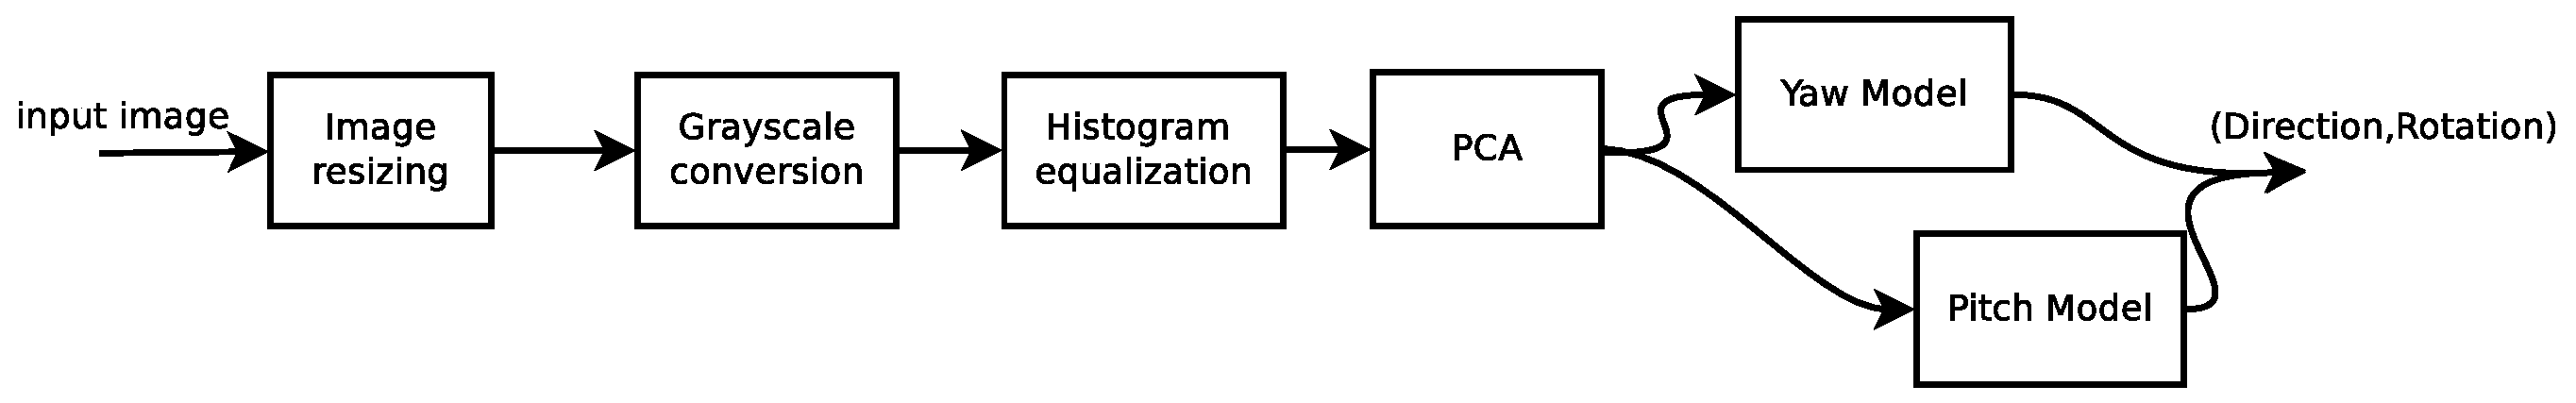
\includegraphics[width=\textwidth]{diagram}
\caption{Schematische voorstelling van het head pose estimation systeem.}
\label{fig:diagram}
\end{figure}

\subsubsection{Voorstelling (feature data)}
 %Dit betekent dat er meer variatie is in de poses die naar rechts kijken dan die naar links kijken. Dit kan eenvoudig opgelost worden door gespiegelde afbeeldingen toe te voegen. 

De trainingsafbeeldingen worden steeds geherscaleerd naar een vaste, kleinere resolutie. 
Verder worden de afbeeldingen ook omgezet naar grijswaarden. %Dit maakt dat elke pixel minder bits bevat en dus het te leren model met minder moet rekening houden. Dit wordt ook zo meestal gedaan in de literatuur.

Hierna wordt er histogramequalisatie toegepast op de afbeelding. Dit zorgt ervoor dat nadelige belichtingseffecten verminderd worden en zorgt voor een globaal beter contrast. 

Vervolgens wordt Principal Component Analysis (PCA) \cite{stat} toegepast. Dit is een statistische methode voor dimensionaliteitsreductie waarbij van $n$ oorspronkelijke (mogelijks gecorreleerde) variablen, $m$ orthogonale variabelen (de zogenaamde principal components, waarbij meestal $m\ll n$) worden gezocht. De eerste principale component verklaart maximaal de covariantie-variantiestructuur, de tweede heeft het tweede grootste aandeel, enzovoort. Geometrisch komt dit overeen met een datatransformatie op een orthogonale basis.

Het selecteren van het aantal componenten is niet heel eenvoudig; deze komen ruwweg overeen met een trade-off tussen rekencomplexiteit en nauwkeurigheid. Het aantal principale componenten werd empirisch vastgelegd op 20, net als in \cite{svmli}.

%Deze variabelen verklaren het meest van de covariantie-variantiestructuur van de trainingset. We kiezen uit de principale componenten de 20 eerste.

% Gabor wavelet, Sobel filter


\subsubsection{Leren van een model}
Na het verwerken van de afbeeldingen van de trainingset wordt deze gebruikt voor het leren van een model.
Bij de neurale netwerk-aanpak wordt er gebruik gemaakt van de ingebouwde neural network (NN) toolbox van Matlab. 
Voor yaw en pitch werd gekozen voor twee afzonderlijke multilayer perceptron NNs, getraind via backpropagation.
%Er is de mogelijkheid om te bepalen hoe een groot deel van de trainingset wordt toegewezen als een trainingset voor het netwerk (en dus welk ander aandeel voor nauwkeurigheid te meten). Op dit trainingssubdeel wordt crossvalidation toegepast en ook deze verhouding kan ingesteld worden. Aangezien we een aparte testset hebben, alloceerden we geen voorbeelden uit de trainingset als testset aan de tool. Verder kan het aantal hidden layers vastgelegd worden.

Voor (LS-)SVM werd LS-SVMlab v$1.7$ gebruikt \cite{suykens2002least}. Ook hier werden de yaw en pitch afzonderlijk behandeld. Als kernel werd voor beide een (Gaussiaanse) RBF kernel gekozen, $K(\boldsymbol{x},\boldsymbol{y})=\exp{(-{\frac{||\boldsymbol{x}-\boldsymbol{y}||^2}{\sigma^2 }})}$, waarbij $\sigma^2$ de squared bandwith is (deze bepaalt de smoothness van de beslissingsoppervlakken \cite{blockeel}). Verder is er nog de regularizatieparameter $\gamma$ die de kost van misclassificaties be\"{\i}nvloedt. Deze parameters kunnen bepaald worden via cross-validation met een grid search of coupled simulated annealing gevolgd door een simplex search.

% Zelf: script voor kiezen parameters itt toolbox van toledo: automatisch via simulated annealing.

\subsubsection{Voorspellen van poses}
Het voorspellen van nieuwe afbeeldingen wordt eenvoudig gedaan door ze te transformeren in dezelfde ruimte als de trainingdata (zie feature data) en deze als invoer te geven aan de niet-lineaire regressiemodellen. 

Aangezien de resultaten van de yaw beter zijn dan die van de pitch,  hebben zij voorrang bij de uiteindelijke bepaling van de pose. Merk op dat we hier gebruik maken van het feit dat we slechts een vrijheidsgraad beschouwen.

\subsection{Evaluatie}
\subsubsection{Neurale netwerken}
Voor neurale netwerken hebben we zowel met als zonder deze extra afbeeldingen getraind. Dit vormt geen probleem aangezien de testafbeeldingen ook binnen die beperkte trainingsrange vallen. Er worden 2 netwerken gebruikt: een voor yaw en een voor pitch.

Tabel~\ref{tabneural} toont parameterinstellingen met de best bekomen resultaten voor enkele iteraties. De parameters zijn volgende:
\begin{itemize}
\item PCA: geeft aan of PCA is toegepast op de afbeelding; indien niet wordt de ruwe afbeelding als feature data gebruikt (na herscalering, omzetting in grijswaarde en hisogramequalisatie).
\item gespiegelde images: geeft aan of de gespiegelde images mee gebruikt worden voor de training of niet.
\item hidden layer (yaw/pitch): geeft de grootte\footnote{Een vuistregel voor de grootte van de hidden layer is dat ze ligt tussen input- en outputgrootte, \cite{hiddenlayer}.}  van de hidden layer in het netwerk voor yaw/pitch.
\item train ratio: geeft het percentage van voorbeelden in de trainingset voor crossvalidation (het complement is het percentage voorbeelden in de validation set).
\end{itemize}

De training gebeurt met een backpropagation conjugate gradient algoritme. De resultaten voor de neurale netwerken vari\"eren sterk in kwaliteit van iteratie tot iteratie. Er zit met een vaste parameterinstelling nog willekeurigheid om tot een concreet netwerk te komen (zoals bijvoorbeeld welke voorbeelden nu net als validation set worden gekozen). 

Het netwerk lijkt (met de geteste parameterinstellingen) over het algemeen het beste te werken zonder de extra afbeeldingen en geeft ook vaker goede resultaten indien we de afbeelding als feature data gebruiken. Maar zonder PCA hebben we een input-grootte van 1024 ($32 \times 32$), wat computationeel wel wat zwaarder is dan met een input-grootte gelijk aan 20 (het gekozen aantal principale componenten).

Wanneer we de resultaten beter bekijken merken we dat soms ook grote classificatiefouten voorkomen. Een voorbeeld voor het model dat overeenstemt met de eerste kolom van tabel~\ref{tabneural} wordt gegeven in figuur ~\ref{bigmistake}.

Goede resultaten kunnen bekomen worden met deze aanpak. Het probleem is dat er meerdere iteraties nodig zijn door de aanwezige randomheid. Ook is het wellicht beter een grotere testset te gebruiken om sluitende conclusies omtrent accuracy te kunnen trekken.

\begin{table}[hbpt] \centering
\begin{tabular} {l S S S S S S} \toprule
PCA 				& {\ding{55}}	& {\ding{55}}	&{\ding{55}}		& {\ding{55}}		& {\ding{51}}		& {\ding{51}}     \\
gespiegelde images 	& {\ding{55}}	& {\ding{55}}	& {\ding{51}} 	& {\ding{51}}		& {\ding{55}}		& {\ding{51}}      \\ \addlinespace

hidden layer (yaw)		& {22}		&{22}			& {22}		& {22}		& {22}		& {22}   \\   
hidden layer (pitch) 	& {25}		& {500}		& {22}		& {22}		& {33}		& {22} \\
train ratio 			& 0.67		& 0.67		& 0.67	& 0.70	& 0.67	& 0.70 \\\midrule

training accuracy (yaw) 	& 0.967	& 0.963	& 0.878	& 0.957	& 0.959	& 0.868\\
training accuracy (pitch) 	& 0.861	& 0.824	& 0.845	& 0.918	& 0.795	& 0.776\\
training accuracy (combined) & 0.828	& 0.787	& 0.724	& 0.875	& 0.7541	& 0.645\\\addlinespace

test accuracy (yaw)	& 0.9		& 0.95	& 0.9		& 0.8		& 1		& 0.8\\
test accuracy (pitch) 	& 0.85	& 0.85	& 0.9		& 0.8		& 0.85	& 0.85\\
test accuracy (combined) 	& 0.75	& 0.8		& 0.8		& 0.6		& 0.85	& 0.65 \\ \bottomrule
\end{tabular}
\caption{Parameters voor NN en training en test accuracies.}
\label{tabneural}
\end{table}

\begin{figure}[hbpt]\centering
	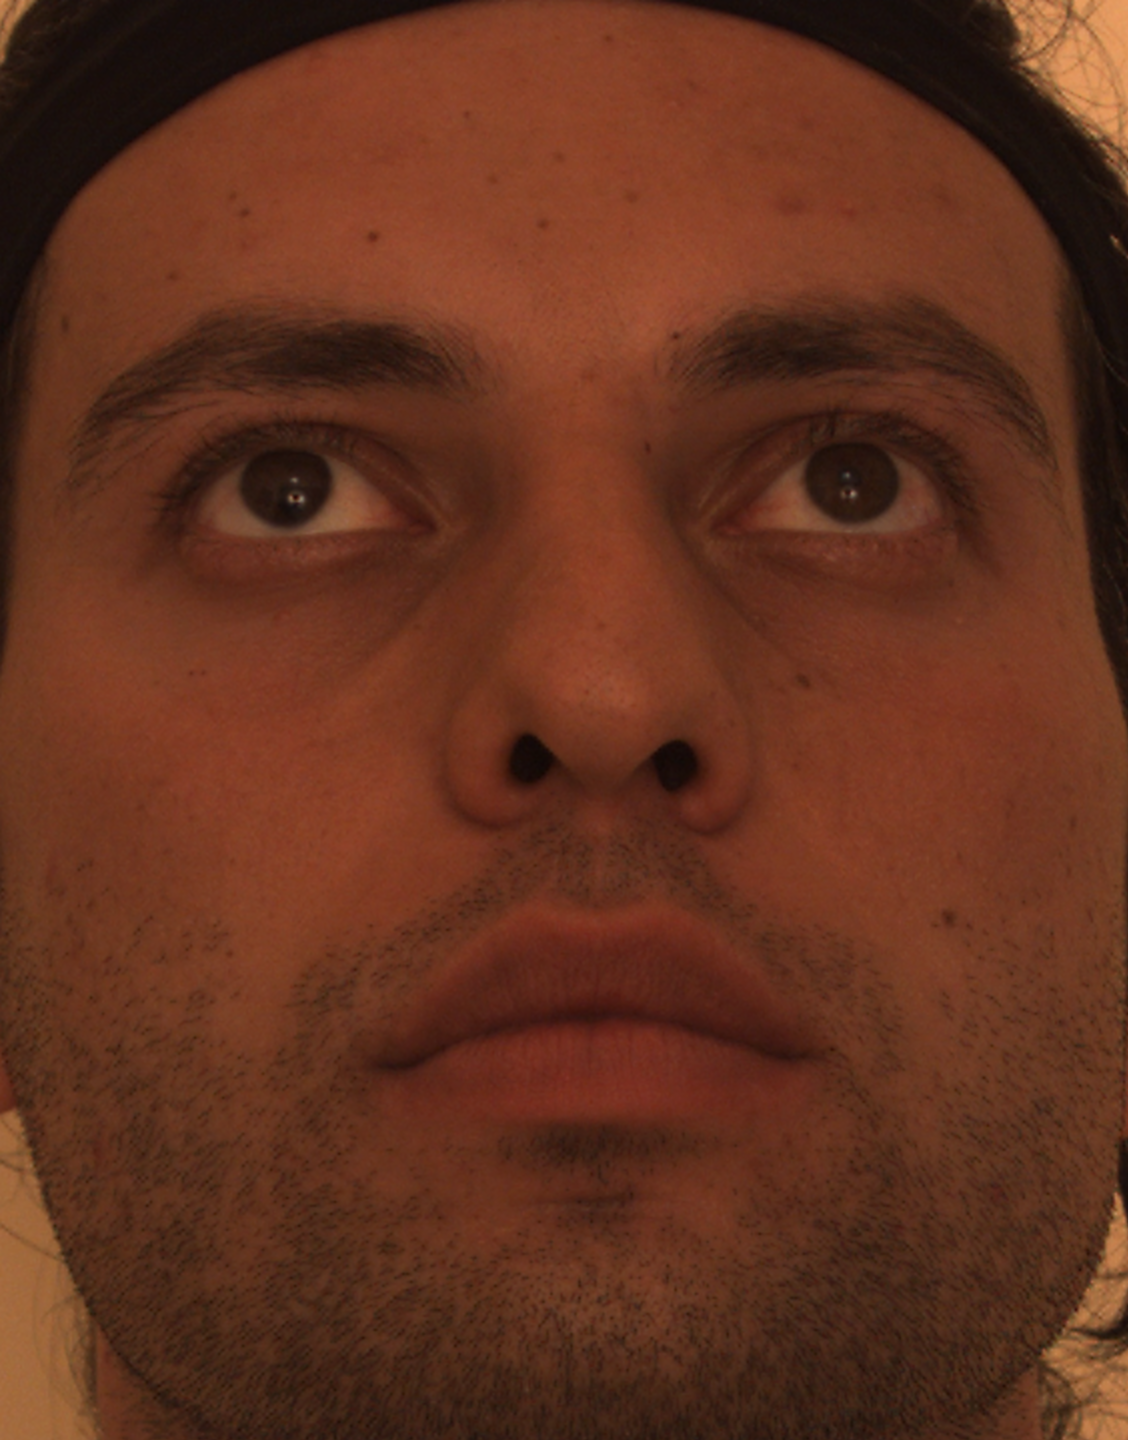
\includegraphics[width=0.3\textwidth]{016}
	\caption{Pose uit de testset die door een NN met een grote fout wordt geclassificeerd (schatting pitch -10\textdegree{} in plaats van 10\textdegree{}).}
	\label{bigmistake}
\end{figure}
\subsubsection{Support Vector Machines}
Tabel~\ref{svmexperiment} toont de parameters voor de kernel van de SVM verkregen via coupled simulated annealing gevolgd door simplex search, en de trainings- en testsetaccuracies. Het is duidelijk dat de nauwkeurigheden op zowel de training- als de testdata algemeen vrij goed zijn.

\begin{table}[hbpt] \centering
\begin{tabular} {l S S S} \toprule
                    &  {$16 \times 16$} & {$32 \times 32$} & {$64 \times 64$} \\ \midrule
$\gamma_{yaw}$ &      0.416 & 2.028  &  3.821     \\
$\sigma^2_{yaw}$ &   7.891&   17.587 &  27.788\\ \addlinespace
$\gamma_{pitch}$ &  165.805 &     1201.045 & 387.463     \\   
$\sigma^2_{pitch}$ & 37.059& 169.826& 73.507 \\ \addlinespace\addlinespace

training accuracy (yaw) &  0.990& 0.987&  0.977\\
training accuracy (pitch) &  0.931& 0.944& 0.954\\
training accuracy (combined) &  0.921& 0.931& 0.931\\\addlinespace

test accuracy (yaw) &       0.95& 1 & 1\\
test accuracy (pitch) & 0.80& 0.85&0.85\\
test accuracy (combined) & 0.75& 0.85&0.85\\ \bottomrule
\end{tabular}
\caption{Parameters voor SVM en training en test accuracies.}
\label{svmexperiment}
\end{table}

Figuur~\ref{fig:fout} toont de 3 foutief geclassificeerde testimages (volgens onze eigen labeling, zie tabel~\ref{tab:label}). Pitch lijkt moeilijker in te schatten dan yaw, zoals ook blijkt uit tabel~\ref{svmexperiment}. Dit is inherent een moeilijker probleem, aangezien de verschillen vergeleken met yawrotaties eerder subtiel zijn. %Het inschatten van pith lijkt ons trouwens ook inherent moeilijker te zijn.

\begin{figure}[hbpt]\centering
\subfloat[P 5\textdegree{} (N)]{\label{f1}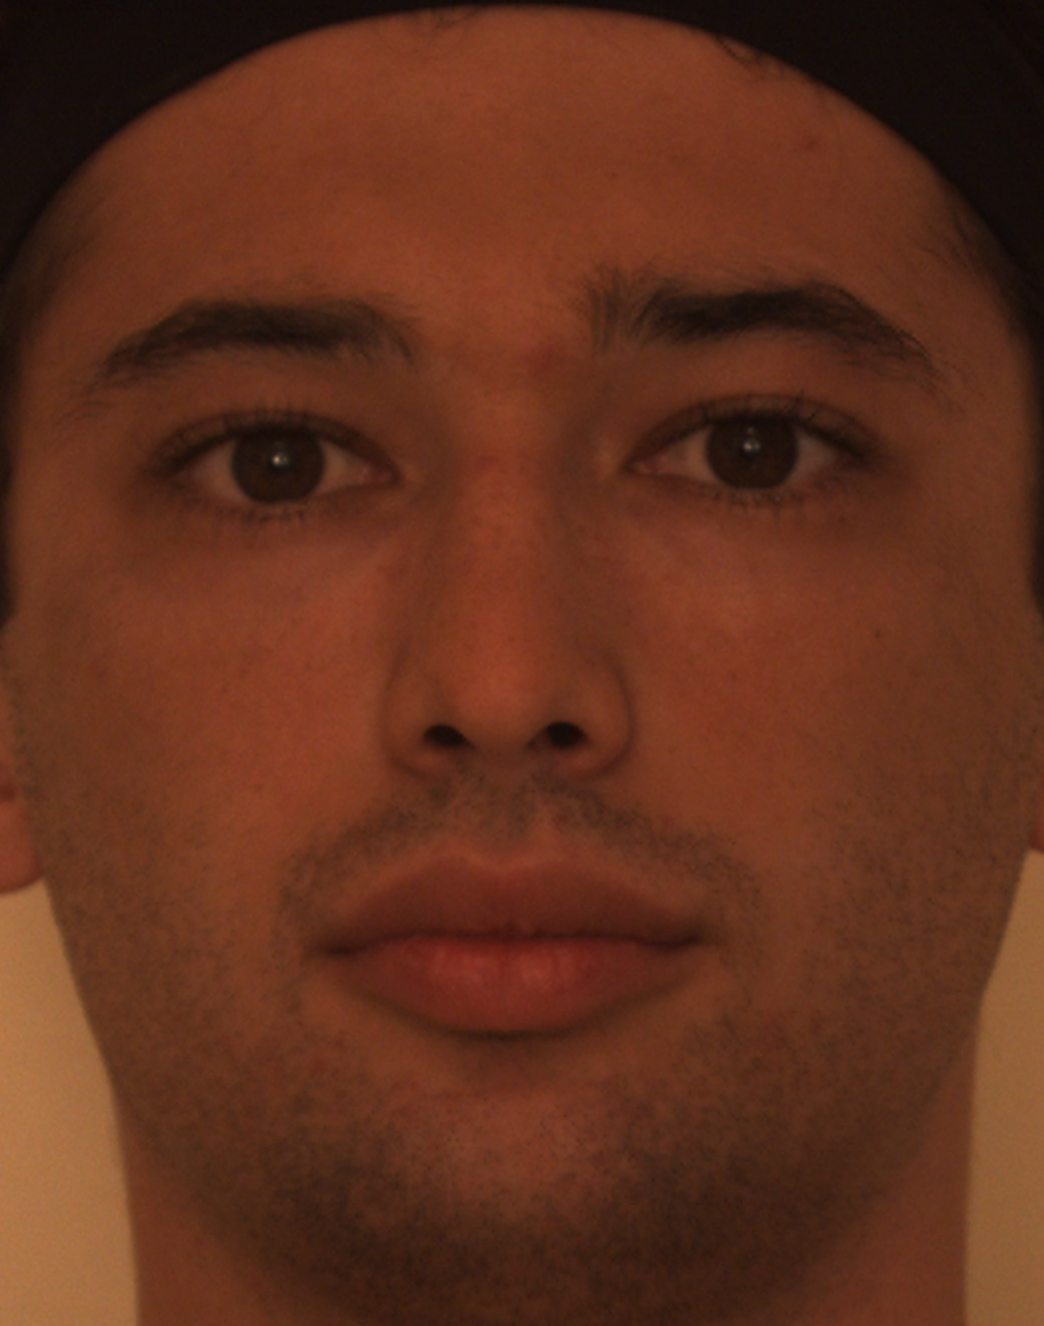
\includegraphics[width=0.22\textwidth]{bs022_N_N_0.png} } \vspace{0.5cm}
\subfloat[P 10\textdegree{} (P 5\textdegree{})]{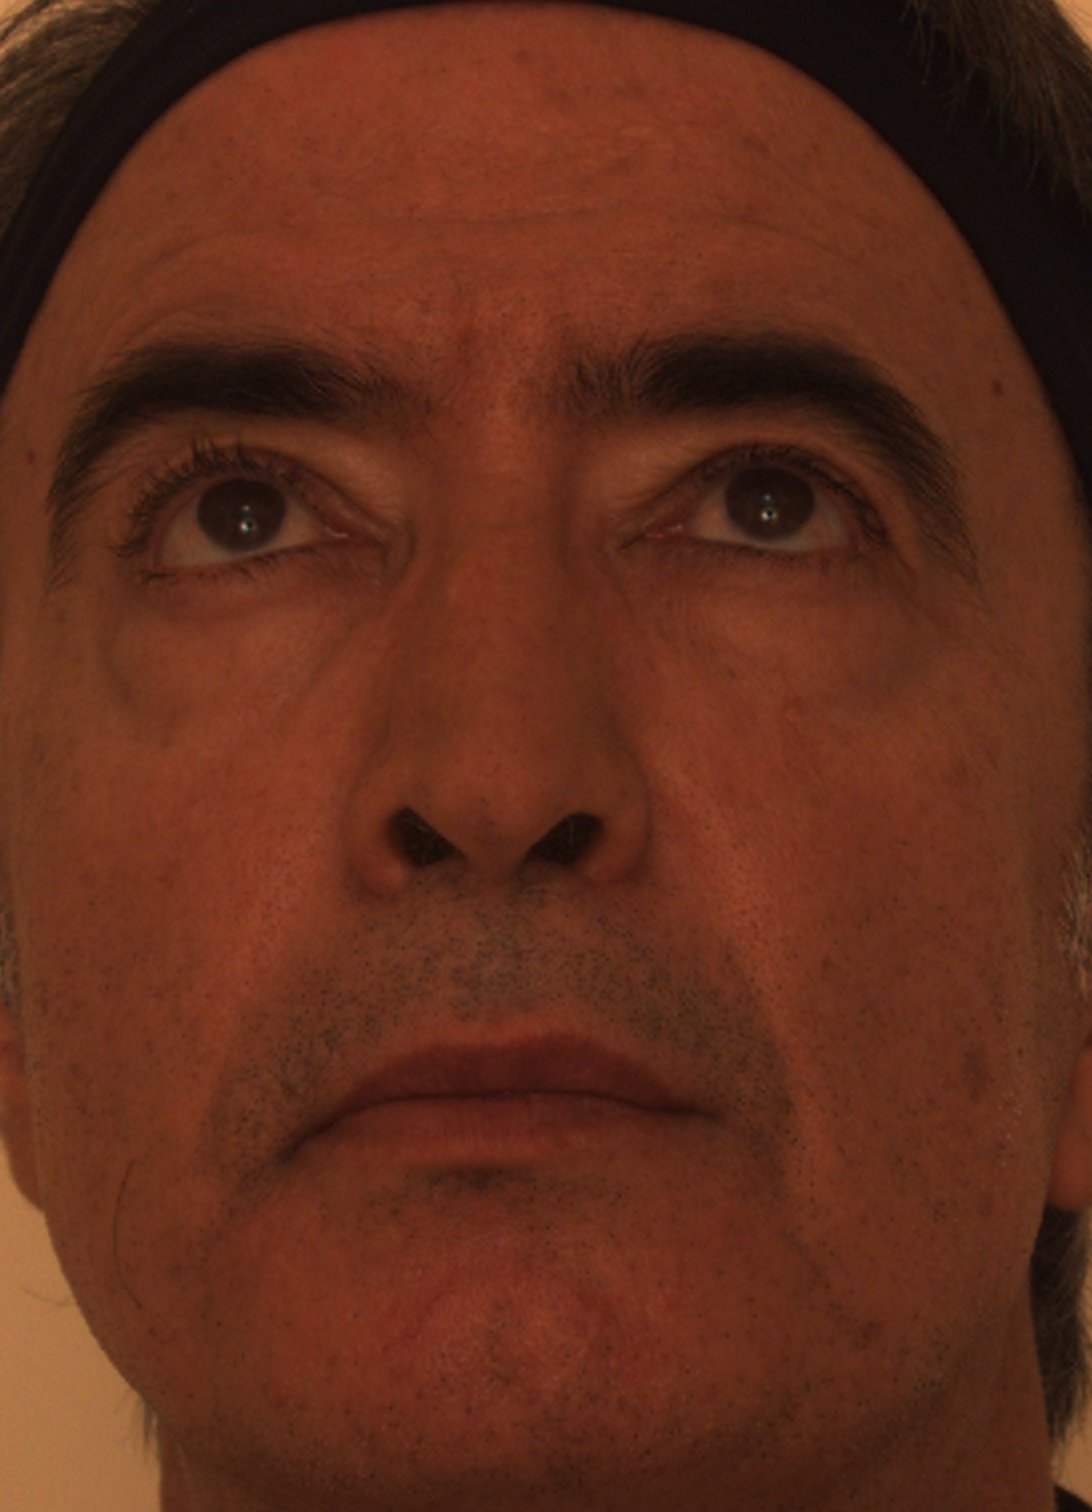
\includegraphics[width=0.22\textwidth]{bs021_PR_SU_0} } \vspace{0.5cm}
\subfloat[N (P 5\textdegree{})]{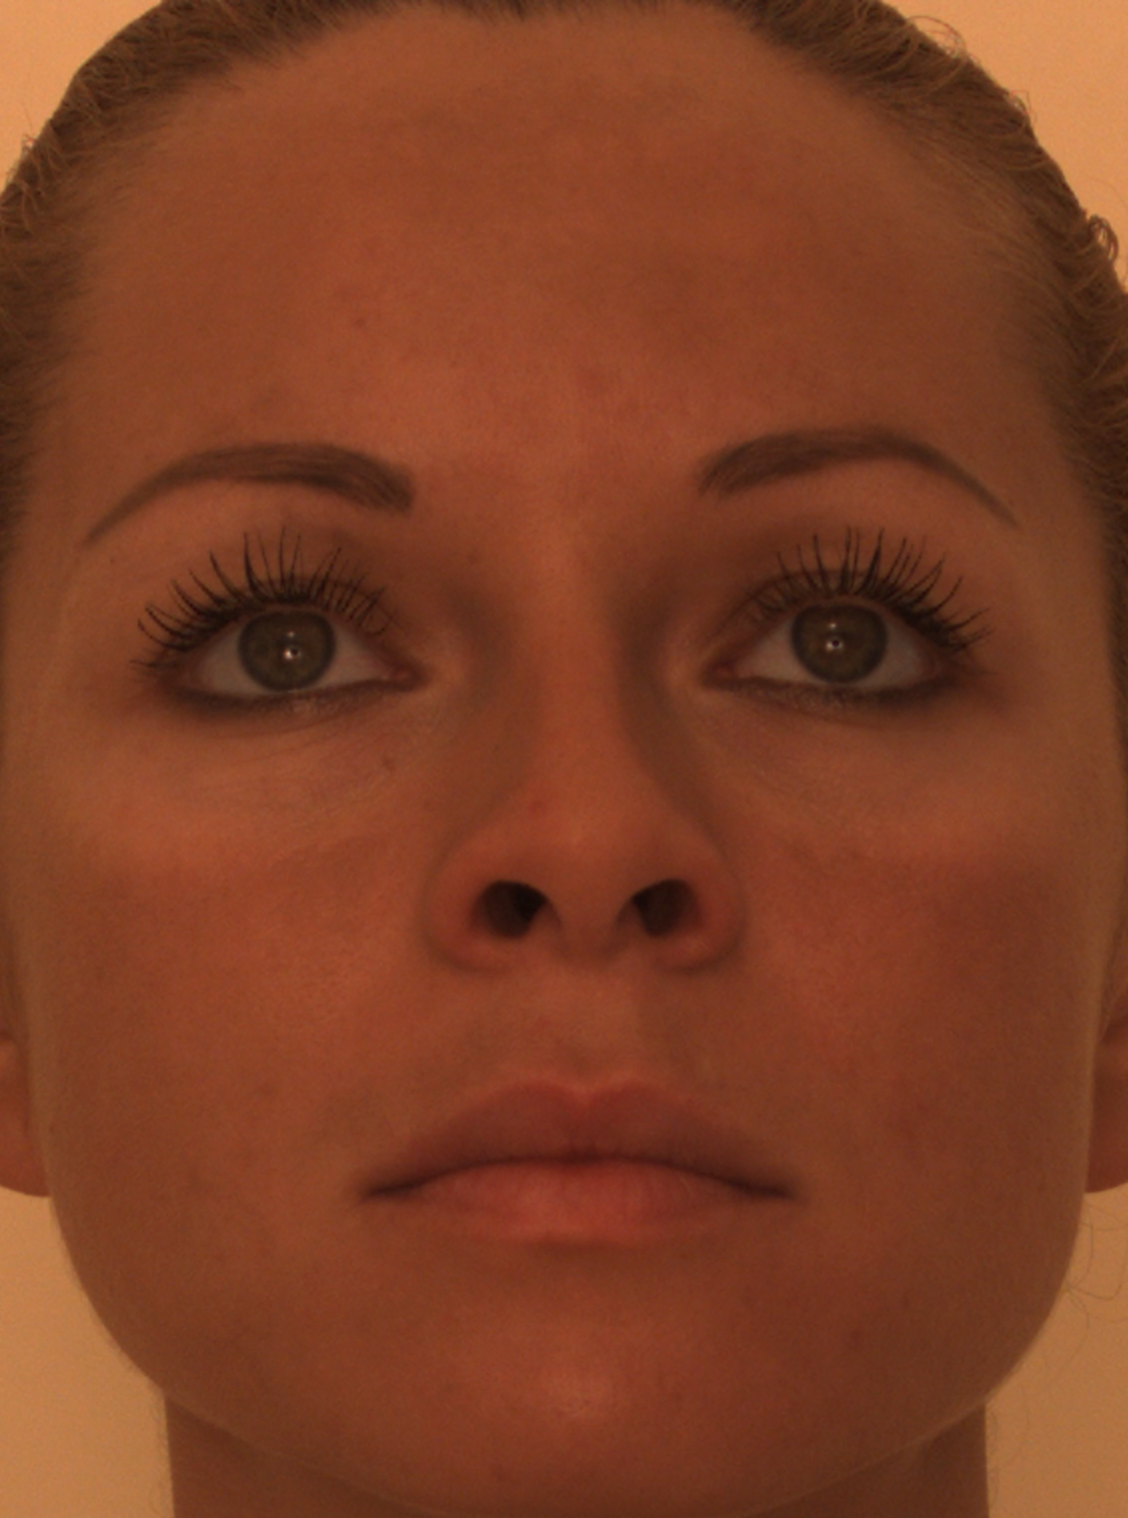
\includegraphics[width=0.22\textwidth]{bs020_PR_SU_0}}\caption{Poses uit de testset die ``verkeerd'' worden voorspeld met SVM. Tussen haakjes staan de ``correcte'' labels.}
\label{fig:fout}
\end{figure}

Het is belangrijk om op te merken dat we geen rekening gehouden met de gradatie van fouten: volledig foute misclassificaties zouden bijvoorbeeld zwaarder kunnen afgestraft worden. Bij onze experimenten is het duidelijk dat als er foute classificaties werden gemaakt, deze slechts een klasse verschilden van de correcte.


\subsubsection{Vergelijking}
Over het algemeen zijn de resultaten van de SVMs dan die van de NNs. De SVMs zijn eenvoudiger te trainen en we bekomen consistent betere nauwkeurigheden voor zowel yaw en pitch (training- en testaccuracy) dan de NNs.

\section{Gezichtsherkenning}
Gezichtsherkenning rekening houdend met posevariatie is geen eenvoudige taak: een overzicht van verschillende aanpakken en hun voor- en nadelen zijn beschreven in \cite{facerec}. Deze paper deelt de methodes in ruwweg 3 categorie\"en: algemene methodes (holistische, lokale algoritmen), 2D (transformatie in pose ruimte) en 3D (gebaseerd op 3D modellen van het hoofd) aanpakken.

\subsection{Implementatie}
Voor het optionele gezichtsherkenning gedeelte hebben we als proof of concept een heel eenvoudig systeem ontwikkeld, gebaseerd op het bekende eigenfaces algoritme \cite{eigenface}.

De stappen zijn in principe heel gelijkaardig aan die voor de pose-estimatie. Hier gebruiken we enkel de neutrale gezichten. Deze worden op analoge manier gepreprocessed en na PCA verkrijgen we een set eigenfaces (zie figuur~\ref{fig:eigenfaces}). We kunnen een nieuw gezicht dan voorstellen als een lineaire combinatie van deze eigenfaces.

\begin{figure}[hbpt]
\centering
 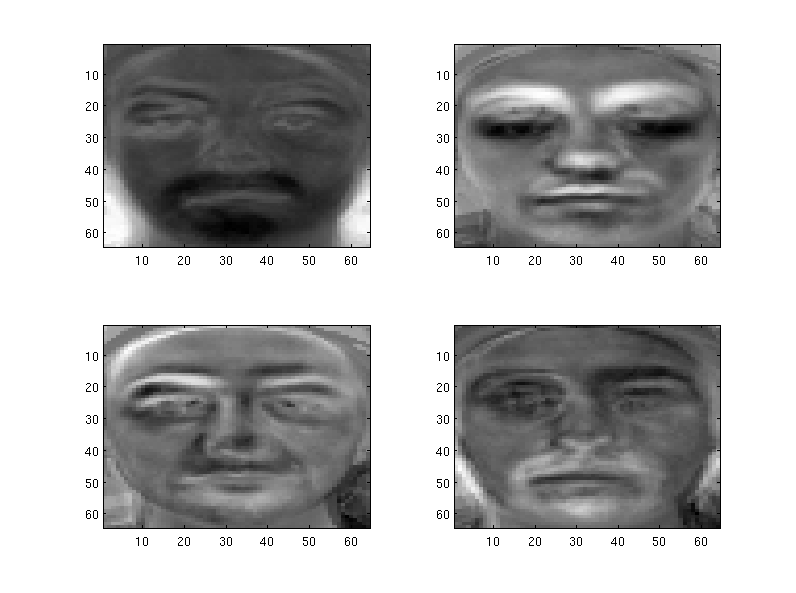
\includegraphics[width=0.6\textwidth]{eigenfaces}
 \caption{Enkele eigenfaces.}
\label{fig:eigenfaces}
\end{figure}

\subsection{Evaluatie}
Voor het voorspellen van gezichten wordt als dissimilariteitsscore gewoon de Euclidische afstand gebruikt (een betere metriek is de Mahalanobis \cite{stat}). Hiermee verkrijgen we een herkenningsrate van 45\% op de gegeven testafbeeldingen. De relatief lage nauwkeurigheid ligt aan het feit dat we momenteel nog geen rekening houden met posevariatie.

Een manier om deze wel in rekening te brengen, is om na het voorspellen van de pose, een virtueel neutraal gezicht te maken (of omgekeerd, de neutrale images omzetten naar de gegeven pose) en deze te vergelijken op bovenstaande manier (een andere mogelijkheid zou kunnen zijn om opnieuw niet-lineaire regressietools te gebruiken). Dit is mogelijk met bijvoorbeeld 3D modellen of Active Appearance Models. Wegens tijdsbeperkingen werden deze extra functionaliteiten echter niet ge\"{\i}mplementeerd. 

Een bijkomstige beperking was overigens dat volgens de specificaties elke te testen afbeelding precies overeenkwam met \'e\'en afbeelding in de database. Dit is uiteraard een na\"{\i}eve veronderstelling en maakt het volledige probleem (personen die niet in de database zitten, posevariatie, onderscheid tussen hoofd en niet hoofd, \ldots{}) heel wat complexer.


\section{Conclusie}
We hebben niet-lineaire regressie gebruikt voor het schatten van de hoofdposes. Als feature data gebruiken we voor een image de geherscaleerde afbeelding ($32 \times 32$), omgezet in grijswaarden en een histogramequalisatie toegepast en ten slotte PCA projectie (20 principale componenten). We hebben een implementatie met neurale netwerken en een met support vector machines vergeleken.

\emph{De support vector machine-aanpak behaalde de beste resultaten}, met een trainingset accuracy van 98\% en 95\% en testset accuracy van 100\% en 85\% voor respectievelijk yaw en pitch.
De gemaakte fouten hierbij waren allen bij pitch en verschilden telkens 1 klasse ten opzichte van de juiste respectieve klasse.

Voor het gezichtsherkenningsysteem hebben we een simpele aanpak gekozen gebaseerd op het eigenfaces algoritme, zonder rekening te houden met de posevariatie. Hiermee krijgen we een gezichtsherkenningsaccuracy van 45\%.
\paragraph{}
Het volledige systeem is uiteraard nog vrij beperkt in mogelijkheden aangezien heel wat vereenvoudigingen werden gemaakt. Zo is er het beperkt aantal rotatievrijheden, de veronderstelling dat alle afbeeldingen hoofden zijn, die reeds mooi werden bijgesneden en van hoge resolutie zijn, zonder hinder van occlusies, \ldots{}

Het lijkt ons interessant om het systeem hiervoor uit te breiden door meer trainingsimages te gebruiken, misschien om heel fijne schattingen te kunnen maken met behulp van bijvoorbeeld Support Vector Regression, evenals Active Appearance Models te gebruiken om gezichten te kunnen synthetiseren zodat het gezichtsherkenningsssyteem hier expliciet gebruik kan van maken. Ook kunnen real-time systemen onderzocht worden. 

Ook hybride vormen die eventueel gebruik maken van de landmarks kunnen mogelijks de moeilijkheden bij het schatten van de pitch verhelpen.


\clearpage

%% Define a new 'leo' style for the package that will use a smaller font.
% \makeatletter
% \def\url@leostyle{%
%   \@ifundefined{selectfont}{\def\UrlFont{\sf}}{\def\UrlFont{\small\ttfamily}}}
% \makeatother
% %% Now actually use the newly defined style.
% \urlstyle{leo}

\bibliography{biblio}

\clearpage

\appendix
\section{Labeling van testdata}
Tabel~\ref{tab:label} toont onze manuele labeling van de testdata. We hebben dit gedaan om ground truth data te hebben om de verschillende experimenten te kunnen beoordelen en te vergelijken. Merk op dat hier waarschijnlijk wat onnauwkeurigheden tussen zitten.
\begin{table}[hbpt] \centering
 \begin{tabular}{l  c r} \toprule
naam & richting & rotatie \\ \midrule
001 &  P &$5$\textdegree{}\\
002& Y &$-90$\textdegree{}\\
003& Y &$30$\textdegree{}\\
004& P &5\textdegree{}\\
005& Y &20\textdegree{}\\
006& Y &30\textdegree{}\\
007& Y &45\textdegree{}\\
008& N &\\
009& P& 10\textdegree{}\\
010& Y& 30\textdegree{}\\
011& Y& 45\textdegree\\
012& Y& 90\textdegree\\
013 & Y& $-45$\textdegree\\
014 & Y& 20\textdegree\\
015 & P& 5\textdegree\\
016 & P& 10\textdegree\\
017 & Y& $-45$\textdegree\\
018 & Y& 10\textdegree\\
019 & Y& 20\textdegree\\
020 & Y& 30\textdegree\\ \bottomrule
 \end{tabular}
\caption{Labeling van testdata.}
\label{tab:label}
\end{table}


\end{document}


	

